\documentclass[11pt]{article}

% Use Helvetica font.
%\usepackage{helvet}

%\usepackage[T1]{fontenc}
%\usepackage[sc]{mathpazo}
\usepackage{color}
\usepackage{amsmath,amsthm,amssymb,multirow,paralist}
\usepackage{graphicx} 
\usepackage{subcaption}
\usepackage{float}

%\renewcommand{\familydefault}{\sfdefault}

% Use 1/2-inch margins.
\usepackage[margin=0.8in]{geometry}
\usepackage{hyperref}


\begin{document}

\begin{center}
{\Large \textbf{Face Mask Detection Using YOLO for Multi-Face Object Detection}

\vspace{10pt}

Project Final Report}

\vspace{10pt}

\textit{By: Gabriel Ferreira}
\end{center}

% \linethickness{1mm}\line(1,0){498}

%%%%%%%%%%%%%%%%%%%%%%%%%%%%%%%%%%%%%%%%%%%%%%%%%%%%%%%%%%%%%%%%%%%%%%%%%%%%%%%

%%%%%%%%%%%%%%%%%%%%%%%%%%%%%%%%%%%%%%%%%%%%%%%%%%%%%%%%%%%%%%%%%%%%%%%%%%%%%%%

\begin{abstract} 
This project aims to develop a computer vision system capable of detecting face masks, an essential task during the COVID-19 pandemic and in post-pandemic contexts where mask-wearing remains relevant for public health and safety. The system is designed to detect multiple faces in images and classify each face into one of three categories: "with mask," "without mask," or "mask weared incorrect." For this purpose, we utilized the Face Mask Detection Dataset from Kaggle for training and evaluation. The YOLO (You Only Look Once) object detection architecture, specifically the YOLO11n variant, was selected for its balance of high accuracy and real-time performance. This implementation supports mask detection across various input sources, including static images, video streams, and live webcam feeds, making it versatile for practical applications. 
\end{abstract}


\section{Introduction} 

Face mask detection has emerged as a critical application in the field of computer vision, particularly during the COVID-19 pandemic when adherence to mask-wearing protocols was vital for curbing the spread of the virus. Even in post-pandemic scenarios, monitoring mask usage remains relevant in settings such as healthcare facilities, public transportation systems, and crowded environments where safety measures are essential. Automating this task using advanced object detection models enables efficient and accurate real-time monitoring.

This project aims to address the challenge of detecting multiple faces in a single frame and classifying each face into one of three categories: "with mask," "without mask," and "mask weared incorrect." To achieve this, we employed the YOLO (You Only Look Once) object detection framework, known for its ability to perform fast and accurate multi-object detection. YOLO’s capability to simultaneously detect and classify multiple objects makes it an ideal solution for real-world face mask detection applications, where multiple individuals may appear within a single image or video frame.

The model chosen for this project is YOLO11n, a lightweight variant of YOLO optimized for both accuracy and real-time performance. Its efficiency allows the system to process input from diverse sources, including static images, pre-recorded videos, and live webcam feeds, making it adaptable to various operational contexts.

The Face Mask Detection Dataset from Kaggle was used for training and evaluation. This dataset includes labeled images of individuals with diverse appearances, lighting conditions, and face orientations, categorized into the three mask-related classes. The diversity of the dataset ensures robust model performance in real-world scenarios.

By leveraging YOLO11n, this project aims to develop a system capable of detecting and classifying face masks with high accuracy while maintaining real-time processing capabilities. The outcomes of this project have potential applications in public safety monitoring, video surveillance systems, and other environments where mask compliance is critical.

\section{Related Work}

YOLO has been widely applied in various object detection tasks due to its real-time detection capabilities. One notable example is its application in automatic license plate recognition, as described in a recent study (Chen, J., \& Su, Y. (2020)). In that project, YOLO was used to detect and extract license plates from images in a fast and efficient manner, even in challenging conditions like low lighting or occlusions. The model's ability to handle these variations and its speed made it an ideal choice for a task where real-time performance is critical.

In the license plate recognition use case, YOLO’s detection framework allowed the model to both localize the plates and classify them in a single pass through the network. This is particularly useful in real-world environments where vehicles may be moving, and the system needs to process frames quickly to capture the license plates in different positions and lighting conditions. The YOLO model used in this project was able to recognize license plates with high accuracy and speed, making it an optimal solution for traffic monitoring systems.

Given YOLO's success in detecting and classifying objects in real-time in the license plate recognition task, it is a strong candidate for the face mask detection problem. Similar to license plates, faces in public spaces may appear in various orientations, positions, and lighting conditions. YOLO’s ability to process images efficiently and detect multiple objects, faces in our case, in a single frame makes it well-suited for our project, where detecting and classifying the mask status of multiple individuals is critical.

\section{Methodology} 
Our approach includes the following key steps:

\subsection{Dataset}
The dataset used in this project is the Face Mask Detection Dataset, sourced from Kaggle. This dataset is specifically curated for face mask detection tasks and provides labeled data to facilitate the training and evaluation of machine learning models. Each image is assigned one of three labels: "with mask," "without mask," or "with mask incorrectly."

The dataset consists of 853 .png images as the input data and .xml files containing corresponding their bounding box annotations and class labels. The XML files follow the Pascal VOC format, which is widely used for object detection tasks and specifies the location of each object in the image along with its associated class. These annotations enable the precise training of models to detect and classify objects within images.

\begin{figure}[H]
    \centering
    \caption{Label Distribution}
    \label{fig:enter-label}
    \includegraphics[width=0.8\linewidth]{project//images/dataset/label_distribution.png} % Increased width
\end{figure}


\subsubsection{Data Sample}
This section presents a visual demonstration of the data used in this project's analysis. The dataset consists of real-world images annotated with bounding boxes that indicate the detection and classification of individuals with our dataset's labels.

\begin{figure}[H]
    \centering
    \caption{Comparison of Original and Labeled Images (Set 1)}
    \label{fig:set1}
    % First pair of images
    \begin{subfigure}[b]{0.48\textwidth} % Increased width slightly
        \centering
        \caption{Image Input}
        \label{fig:input1}
        \includegraphics[width=\textwidth]{images/dataset/maksssksksss0.png}
    \end{subfigure}
    \hspace{0.02\textwidth} % Reduced spacing between images
    \begin{subfigure}[b]{0.48\textwidth} % Increased width slightly
        \centering
        \caption{Image Input With Plotted Labels}
        \label{fig:output1}
        \includegraphics[width=\textwidth]{images/dataset/maksssksksss0_labeled.png}
    \end{subfigure}
\end{figure}

\begin{figure}[H]
    \centering
    \caption{Comparison of Original and Labeled Images (Set 2)}
    \label{fig:set2}
    % Second pair of images
    \begin{subfigure}[b]{0.48\textwidth} % Increased width slightly
        \centering
        \caption{Image Input}
        \label{fig:input2}
        \includegraphics[width=\textwidth]{images/dataset/maksssksksss786.png}
    \end{subfigure}
    \hspace{0.02\textwidth} % Reduced spacing between images
    \begin{subfigure}[b]{0.48\textwidth} % Increased width slightly
        \centering
        \caption{Image Input With Plotted Labels}
        \label{fig:output2}
        \includegraphics[width=\textwidth]{images/dataset/maksssksksss786_labeled.png}
    \end{subfigure}
\end{figure}



\subsubsection{Data Preprocessing}

To prepare the dataset for YOLO11n training, the Pascal VOC XML annotations were converted into the YOLO format. The YOLO annotation format represents each bounding box as normalized coordinates $(x_{center}, y_{center}, width, height)$ along with the class label. Each image has a corresponding .txt file containing these annotations, with each line representing one object in the image. 

The final step involved organizing the dataset into the folder hierarchy expected by YOLO11n: images were stored in an \textit{images} folder, and their corresponding labels were saved in a separate \textit{labels} folder. This structure ensures compatibility with YOLO11n's training pipeline.

The conversion process included the following steps:

\begin{enumerate} 
    \item Parsing the XML files to extract bounding box coordinates and class labels. 
    \item Normalizing the bounding box coordinates relative to the image dimensions. 
    \item Writing the converted annotations into .txt files, ensuring each .txt file matches its corresponding label file name. 
    \item Storing all .png files in the \textit{images} folder and all .txt files in the \textit{labels} folder.
\end{enumerate}

This conversion process was automated using a custom preprocessing script to maintain consistency and efficiency across the dataset. The resulting YOLO compatible dataset ensured the integration with the YOLO11n training pipeline and eliminated manual intervention in the data preparation phase. This streamlined approach also minimized the risk of errors, making the training process more reliable.

\subsubsection{Data Split}
The dataset is pre-split into training, evaluation, and testing sets to ensure a clear separation of data for model development and performance evaluation. This structured split supports effective training while providing unbiased performance metrics on unseen data.

\begin{itemize}
    \item Training Set ($70\%$): The largest subset of the data, used to optimize the model parameters. It includes a diverse array of images featuring individuals from various demographics, captured under different lighting conditions, angles, and face orientations. This diversity ensures that the model learns robust features applicable to real-world scenarios.
    \item Evaluation Set ($10\%$): A smaller subset of the data, used during training to monitor the model’s performance and fine-tune hyperparameters. This set helps in early detection of overfitting or underfitting by evaluating the model on data it has not been directly trained on.
    \item Testing Set ($20\%$): A separate and unseen subset reserved for the final evaluation of the model's performance. It provides an unbiased assessment of the model’s generalization capabilities and is used to measure metrics like precision, recall, and overall accuracy.
\end{itemize}

The dataset's inherent diversity in demographics, environmental conditions, and face orientations plays a crucial role in ensuring that the model is well-suited for deployment in dynamic, real-world conditions. The careful separation of data subsets minimizes data leakage and allows for reliable benchmarking of the model’s performance.

\subsection{Data Modeling}
\subsubsection{Training the YOLO Model}
The YOLO v11 size n model was retrained using transfer learning, leveraging pretrained weights as a foundation and fine-tuning the model on the Face Mask Detection Dataset. This approach takes advantage of the model’s existing knowledge from large-scale object detection tasks while adapting it to the specific task of face mask detection.

The training process involved several key steps:
    \begin{itemize}
        \item \textbf{Transfer Learning -}
        The pretrained weights of YOLO v11n, trained on a large and diverse dataset (e.g., COCO), were used as a starting point. Transfer learning significantly reduces the training time and computational resources required while improving model performance by retaining learned features such as edge detection, object boundaries, and general shapes.
        \item \textbf{Training Configuration -}
        To fine-tune the model, specific training configurations were adjusted to suit the face mask detection task:
            \begin{itemize}
                \item \textbf{Input Size:} YOLO v11n is optimized for real-time processing, maintaining a balance between accuracy and speed by using a compact input resolution suitable for face detection.
                \item \textbf{Number of Epochs:} The training process was conducted incrementally, starting with 50 epochs in the initial experiments and progressively increasing the number of epochs based on the model's performance and convergence behavior. At each stage, we experimented with different techniques, such as learning rate adjustments, data augmentation strategies, and hyperparameter tuning. These techniques will be further detailed in the Experimental Results section. This iterative approach allowed us to refine the training process and achieve better performance while avoiding excessive training time in early stages.
                \item \textbf{Early Stopping:} Early stopping was implemented to dynamically control the number of epochs, preventing overfitting and ensuring efficient training. Validation loss and mAP metrics (more on this in the Metrics section) on the evaluation set were monitored during each training session. Training was halted if the validation loss failed to improve for 5 consecutive epochs. This approach ensured that we could experiment with incremental training without wasting computational resources on overfitting.
                \item \textbf{Batch Size:} The batch size was set based on the dataset size and available GPU memory, ensuring stable training updates.
                \item \textbf{Data Augmentation:} Techniques such as random horizontal flipping, scaling, and brightness adjustments were applied to improve the model's robustness to variations in real-world conditions.
            \end{itemize}
    \item \textbf{Hardware and Framework -} The initial attempt to train the YOLO v11n model was performed locally on a MacBook with an Intel processor. However, this approach proved to be inefficient as older MacBook models lack GPU compute capabilities, significantly slowing down the training process for deep learning models. Training deep learning models without GPU acceleration often results in impractically long training times, making it unsuitable for this project’s requirements.
    
    To overcome these limitations, the project utilized the Google Colab environment, which provides free, time-limited, access to GPU resources. By leveraging Google Colab, the training process was significantly accelerated, enabling the effective fine-tuning of the YOLO v11n model.
    
    The training environment leveraged the following key resources:
    \begin{itemize} 
        \item \textbf{Hardware:} NVIDIA GPU provided by Google Colab for accelerated training, ensuring efficient handling of large datasets and computationally intensive model updates. 
        \item \textbf{Framework:} PyTorch implementation of YOLO v11n, seamlessly integrated with the Ultralytics library. The library provided an intuitive interface for configuring the model, managing datasets, and monitoring training progress. 
    \end{itemize}

The combination of Google Colab's GPU capabilities and PyTorch’s flexibility allowed the project to overcome local hardware constraints and achieve efficient training workflows. This setup ensured the model could be fine-tuned within a reasonable timeframe while maintaining accuracy and real-time performance objectives. Future work may explore using dedicated cloud-based GPUs for more extensive training and experimentation.
    \end{itemize}


\subsubsection{Evaluation Metrics}
The performance of the YOLO v11n model was evaluated using a combination of standard metrics commonly used in object detection tasks. These metrics provided a comprehensive understanding of the model's accuracy, robustness, and ability to generalize across different classes. The following metrics were utilized:

\begin{itemize} 
    \item \textbf{Precision, Recall, and F1-Score:} These metrics evaluate the balance between the correctness of predictions (Precision) and the coverage of true positives (Recall). F1-Score provides a harmonic mean of Precision and Recall.
    \[
    \text{Precision} = \frac{\text{TP}}{\text{TP} + \text{FP}}, \quad
    \text{Recall} = \frac{\text{TP}}{\text{TP} + \text{FN}}, \quad
    F1 = 2 \cdot \frac{\text{Precision} \cdot \text{Recall}}{\text{Precision} + \text{Recall}}
    \]

    \item \textbf{Intersection over Union (IoU):} Measures the overlap between predicted and ground truth bounding boxes.
    \[
    \text{IoU} = \frac{\text{Area of Overlap}}{\text{Area of Union}}
    \]

    \item \textbf{Mean Average Precision (mAP):} The primary evaluation metric for object detection, mAP measures the area under the precision-recall curve across IoU thresholds. This project calculates mAP at IoU thresholds of 0.5 (mAP@0.5) and 0.5:0.95 (mAP@[0.5:0.95]).
    \[
    \text{AP} = \int_0^1 \text{Precision}(\text{Recall}) \, d(\text{Recall)}, \quad
    \text{mAP} = \frac{1}{n} \sum_{i=1}^{n} \text{AP}_i
    \]

    \item \textbf{Inference Speed (Frames Per Second):} Assesses real-time performance in dynamic environments.
\end{itemize}

These metrics were calculated on the test dataset, ensuring an unbiased assessment of the model’s performance. The combination of mAP and class-specific metrics provided detailed insights into the model’s strengths and areas for improvement.


\section{Experimental Results}
This section describes the results of the key experiments conducted during the training and evaluation phases. While several experiments were performed throughout the project, only the most impactful ones are presented here to highlight the progression of the model's performance and the underlying reasoning behind each iteration. These experiments illustrate how adjustments to hyperparameters, input configurations, and training strategies influenced the metrics and qualitative observations. Each experiment is characterized by unique configurations, and their results include training and testing metrics, along with prediction samples for visualization.

\subsubsection{Experiment 1 and 2 - Baseline Model}
The first experiment represents the baseline configuration, where the YOLO v11n model was trained with default pretrained weights and minimal hyperparameter tuning. This experiment served as a starting point for evaluating the model's performance on the Face Mask Detection Dataset without any modifications or optimizations. The goal of this experiment was to establish a benchmark for future experiments.

\begin{itemize}
    \item \textbf{Key configurations included:}   
    \begin{itemize} 
        \item \textbf{Learning Rate:} 0.01 (default) 
        \item \textbf{Batch Size:} 64 \item \textbf{Epochs:} 100 (50 + 50) 
        \item \textbf{Data Augmentation:} None (default)
        \item \textbf{Image Size}: 640
        \item \textbf{Early Stopping}: 100 (default)
    \end{itemize}

    \item \textbf{Train Metrics:} Training mAP@0.5: 72.2\% 

        \begin{figure}[H]
            \centering
            \caption{Training Losses}
            \label{fig:enter-label}
            \includegraphics[width=0.9\linewidth]{project//images/train_yolo11n_v2/results.png} % Increased width
        \end{figure}

        \begin{figure}[H]
            \centering
            \caption{Comparison of Precision and Recall Confidence Curve}
            \label{fig:set1}
            % First pair of images
            \begin{subfigure}[b]{0.48\textwidth} % Increased width slightly
                \centering
                \includegraphics[width=\textwidth]{project/images/train_yolo11n_v2/P_curve_mod.png}
            \end{subfigure}
            \hspace{0.02\textwidth} % Reduced spacing between images
            \begin{subfigure}[b]{0.48\textwidth} % Increased width slightly
                \centering
                \includegraphics[width=\textwidth]{project/images/train_yolo11n_v2/R_curve_mod.png}
            \end{subfigure}
        \end{figure}

    \item \textbf{Test Metrics:} Testing mAP@0.5: $69.5\%$

        \begin{figure}[H]
            \centering
            \caption{Confusion Matrix}
            \label{fig:enter-label}
            \includegraphics[width=.9\linewidth]{project//images/train_yolo11n_v2/val/confusion_matrix_normalized.png} % Increased width
        \end{figure}

        \begin{figure}[H]
            \centering
            \caption{Comparison of Original and Labeled Images (Set 1)}
            \label{fig:set1}
            % First pair of images
            \begin{subfigure}[b]{0.48\textwidth} % Increased width slightly
                \centering
                \caption{Batch Labels}
                \label{fig:input1}
                \includegraphics[width=\textwidth]{project/images/train_yolo11n_v2/val/val_batch1_labels.jpg}
            \end{subfigure}
            \hspace{0.02\textwidth} % Reduced spacing between images
            \begin{subfigure}[b]{0.48\textwidth} % Increased width slightly
                \centering
                \caption{Batch Predictions}
                \label{fig:output1}
                \includegraphics[width=\textwidth]{project/images/train_yolo11n_v2/val/val_batch1_pred.jpg}
            \end{subfigure}
        \end{figure}    

    \item \textbf{Qualitative Observations:}
        \begin{itemize}
            \item The model performed reasonably well in detecting single faces in images and accurately classifying "with mask" and "without mask" labels.
            \item However, it struggled significantly with multi-face scenarios, especially for the "mask weared incorrect" class. This issue was likely due to a lack of augmentation and the relatively small input image size, which limited the model’s ability to resolve finer details.
            \item False positives were observed in background regions, highlighting the need for better generalization.
        \end{itemize}
\end{itemize}

\subsubsection{Experiment 4 - Image Size Input Amplified} This experiment was conducted based on insights from earlier experiments, where the default input image size appeared to limit the model's performance, particularly for detecting small objects or resolving fine details. The input image size was increased to 1024, while other configurations were incrementally fine-tuned. This experiment achieved notable metric improvements and was selected as the best-performing configuration for the final presentation.

\begin{itemize}
    \item \textbf{Key configurations included:}   
    \begin{itemize} 
        \item \textbf{Learning Rate:} 0.01 (default) 
        \item \textbf{Batch Size:} 32 \item \textbf{Epochs:} 200 (150 + 50) 
        \item \textbf{Data Augmentation:} None (default)
        \item \textbf{Image Size}: 1024
        \item \textbf{Early Stopping}: 100 (default)
    \end{itemize}

    \item \textbf{Train Metrics:} Training mAP@0.5: 80.02\% 

        \begin{figure}[H]
            \centering
            \caption{Training Losses}
            \label{fig:enter-label}
            \includegraphics[width=0.9\linewidth]{project//images/train_yolo11n_v4/results.png} % Increased width
        \end{figure}

        \begin{figure}[H]
            \centering
            \caption{Comparison of Precision and Recall Confidence Curve}
            \label{fig:set1}
            % First pair of images
            \begin{subfigure}[b]{0.48\textwidth} % Increased width slightly
                \centering
                \includegraphics[width=\textwidth]{project/images/train_yolo11n_v4/P_curve_mod.png}
            \end{subfigure}
            \hspace{0.02\textwidth} % Reduced spacing between images
            \begin{subfigure}[b]{0.48\textwidth} % Increased width slightly
                \centering
                \includegraphics[width=\textwidth]{project/images/train_yolo11n_v4/R_curve_mod.png}
            \end{subfigure}
        \end{figure}

    \item \textbf{Test Metrics:} Testing mAP@0.5: $72.7\%$

        \begin{figure}[H]
            \centering
            \caption{Confusion Matrix}
            \label{fig:enter-label}
            \includegraphics[width=.9\linewidth]{project//images/train_yolo11n_v4/val/confusion_matrix_normalized.png} % Increased width
        \end{figure}

        \begin{figure}[H]
            \centering
            \caption{Comparison of Original and Labeled Images (Set 1)}
            \label{fig:set1}
            % First pair of images
            \begin{subfigure}[b]{0.48\textwidth} % Increased width slightly
                \centering
                \caption{Batch Labels}
                \label{fig:input1}
                \includegraphics[width=\textwidth]{project/images/train_yolo11n_v4/val/val_batch1_labels.jpg}
            \end{subfigure}
            \hspace{0.02\textwidth} % Reduced spacing between images
            \begin{subfigure}[b]{0.48\textwidth} % Increased width slightly
                \centering
                \caption{Batch Predictions}
                \label{fig:output1}
                \includegraphics[width=\textwidth]{project/images/train_yolo11n_v4/val/val_batch1_pred.jpg}
            \end{subfigure}
        \end{figure}    

    \item \textbf{Qualitative Observations:}
        \begin{itemize}
            \item The increase in input image size significantly improved the model’s detection and classification performance across all classes, with a particular improvement for the "mask weared incorrect" class.
            \item The model exhibited fewer false positives in background regions, suggesting better generalization to unseen data.
            \item This configuration provided the best balance of precision and recall observed during the project. It was chosen for the final presentation due to its superior overall performance.
            \item There are a lot of areas for improvement still.
        \end{itemize}
\end{itemize}

\section{Conclusion}

This project successfully demonstrated the application of the YOLO v11n object detection model for face mask detection. Through iterative experimentation, I explored the impact of various hyper-parameters, input configurations, and training strategies. Each experiment provided valuable insights into the strengths and limitations of the model, allowing me to refine it for better performance.

One of the most significant findings was the impact of increasing the input image size, which led to notable improvements in both quantitative metrics (mAP@0.5) and qualitative performance. The best-performing model achieved a testing mAP@0.5 of 72.7\%, with a significant reduction in false positives and enhanced detection of the challenging "mask weared incorrect" class. This highlighted the importance of balancing model configurations to optimize accuracy while maintaining generalization.

However, one of the major challenges encountered was the issue of unbalanced labels in the dataset. The "with mask" class was overrepresented compared to the "without mask" and "mask weared incorrect" classes. This imbalance caused the model to struggle with detecting and classifying the less frequent class accurately, as it had fewer examples to learn from during training. Efforts such as increasing input image size and conducting targeted evaluation helped mitigate some of these effects, but they remained a limitation of the current implementation. In future work, techniques like class weighting, synthetic data generation, intentionally increasing the samples containing less frequent classes in the training set, or oversampling the minority class could be explored to address this imbalance and further improve the model's robustness.

Despite these challenges, this project showcased the effectiveness of YOLO for real-time face mask detection, with practical applications in public safety and healthcare. The skills and knowledge I gained from this project, including dataset preparation, model training, and performance evaluation, will be invaluable for tackling future challenges in computer vision and deep learning.

\section{Future Plan}

This project has laid a solid foundation for real-time face mask detection using the YOLO v11n model. However, there are several areas where further improvements and extensions can be explored to enhance the system’s performance and practicality. Below are the key steps planned for the future:

\begin{enumerate}
    \item \textbf{Addressing Data Imbalance:}
    \begin{itemize}
        \item Implement techniques to handle the imbalance between the "mask worn incorrectly" class and the other two classes. Potential approaches include:
        \begin{itemize}
            \item \textbf{Class Weighting:} Assigning higher weights to the minority class during training.
            \item \textbf{Oversampling:} Increasing the number of samples for the minority class through duplication or synthetic data generation.
            \item \textbf{Data Augmentation:} Applying targeted augmentation to underrepresented classes to improve their representation in the training set.
        \end{itemize}
    \end{itemize}

    \item \textbf{Incorporating Advanced Data Augmentation:}
    \begin{itemize}
        \item Explore augmentation techniques such as random rotations, perspective transformations, and adding synthetic noise to improve the model’s robustness to diverse real-world conditions.
    \end{itemize}

    \item \textbf{Exploring YOLO Variants:}
    \begin{itemize}
        \item Experiment with newer YOLO variants (e.g., YOLOv8 or YOLOv11x) that may provide better accuracy and speed trade-offs.
    \end{itemize}

    \item \textbf{Improving Real-Time Performance:}
    \begin{itemize}
        \item Measure and improve inference speed (frames per second) while maintaining high accuracy.
    \end{itemize}

    \item \textbf{Deploying a Complete System:}
    \begin{itemize}
        \item Develop an end-to-end system that integrates the model with video feeds and provides real-time statistics, including:
        \begin{itemize}
            \item \textbf{Count of People:} Total individuals detected in a frame.
            \item \textbf{Label Distribution:} Real-time percentage of each mask-related class.
        \end{itemize}
        \item Incorporate an alert system to notify users when individuals are detected without masks or wearing masks incorrectly.
    \end{itemize}
\end{enumerate}

These steps will further enhance the accuracy, robustness, and applicability of the system, making it more suitable for deployment in dynamic real-world environments. By addressing the current challenges and leveraging advanced techniques, the model can become a reliable tool for public safety and healthcare monitoring.
\newpage


\section{References}

\begin{enumerate}
    \item Kaggle, “Face Mask Detection Dataset,” available at: \newline
    https://www.kaggle.com/datasets/andrewmvd/face-mask-detection.
    \item Chen, J., \& Su, Y. (2020). YOLO-Based License Plate Recognition Algorithm. Journal of Computer Engineering and Applications, 45(2).
\end{enumerate}


\end{document}
